\section{Hardware components}
In the very beginning of the project, the team looked into the possibility of getting live data directly from devices. This required some technical equipment for collecting and transmitting the power usage from a device. The original idea was that the app should get data directly form the devices in the house, and if possible control the devices.

\todo{The team concluded that the only reasonable architecture for a fully automatic measurement would include a small server, running on a Raspberry Pi, and one measurement device with wireless transmitter connected to anything the user wanted to control and monitor. These particular devices that allow for wireless transmission proved to be hard to find as they have not achieved much success on the market. Much of this is due to the lack of standards in transmission between devices and servers. The team found that many of the existing apps would have a device that were desired, but that it would be proprietary technology. The customer had previously requested that the devices should be cheap and preferably based on open source technology. As mentioned, all these challenges combined with time constraints lead the team, in agreement with the customer, to develop the app without supporting this. Instead the app was to be developed in way to would allow easy integration of this functionality at a later point in time. More details on this can be found in chapter~\ref{sec:further}, along with more about how the team envisions further development. }

\subsection{Home data aggregator}
To ensure full operability 24 hours a day, a base station is needed in the user's home. This server will serve as an aggregating agent for data from measuring units attached to devices. Given an ideal architecture implementation, this unit would also be responsible for controlling devices. The team envisions this unit as a REST service mostly running synchronizations towards the Wattitude cloud server.\todo{<- Bør endres på} The software for such a server could be based on the current server software. The hardware for a this base station would be as simple as a Raspberry pi\cite{pi}. These computers are small, cheap and provides all the hardware needed for a simple home aggregator. Some modifications might be necessary to communicate with the measuring units. The architecture for this aggregation unit is shown in figure~\ref{fig:aggregator}.

\begin{figure}[H]
\centering
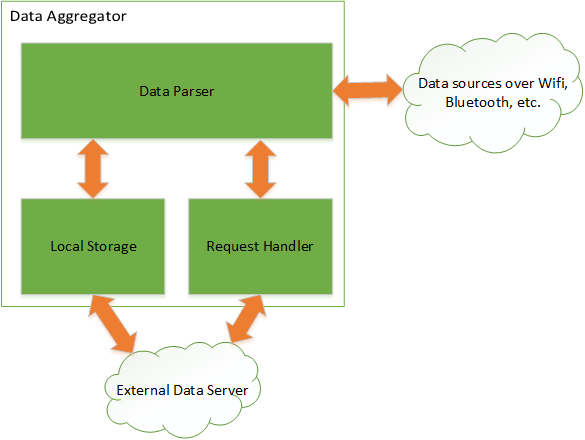
\includegraphics[height=0.4\textheight]{ch/further/fig/home.png}
\caption{Detailed architecture for the home data aggregator.}
\label{fig:aggregator}
\end{figure}

\subsection{Measuring unit}
To make real time monitoring possible, every device that the user wants to monitor must be connected to a wireless monitoring unit. The team tried to find an existing solution that was satisfying, but most of the options we found was proprietary and/or to expensive. The following paragraphs describes the most viable options.

\paragraph{HomeMatic plug}
This is the device that the Cossmic team at Sintef has been experimenting with. The first drawbacks are that it must be ordered from Germany, and that it has a unit price of almost 500NOK. Covering most home devices with such a measuring device would be extremely costly. It is part of the HomeMatic proprietary hardware line, and is meant to interface with a HomeMatic central control unit, much like the base station we have described above. As hardware devices were not a part of the project scope, the team did not do any research on how to interface with this unit. The only knowledge we have is that the Sintef team working on Cossmic has been working on it.

\paragraph{Do It Yourself(DIY) Arduino}
A much cheaper, but perhaps limited solution is one from Open Energy Monitor~\cite{oemmodule}. These units do not support control of devices, only measurement of consumption. They are much cheaper than the HomeMatic unit, but must be assembled manually. This unit can be good for experimenting and prototyping but it is not ready for the home market.